% \subsection{Sampling Behavior of Buffers} \label{subsec:buffer_eval}

% To validate the sampling behavior of the implemented buffers, \autoref{fig:buffer} shows the sample frequency for each added time step over 100 samples. The results are generated by adding experiences until the buffer is full. Additionally, \ac{PER} and \ac{BPER} get random \ac{TD}-errors and rewards per experience, to model the expected behavior.

% \begin{figure}[h]
%     \centering
%     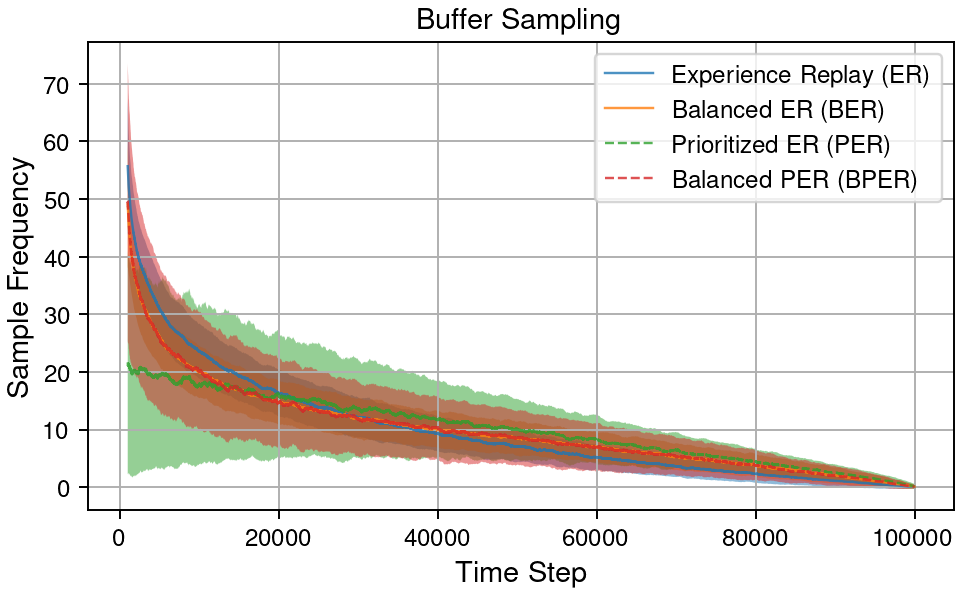
\includegraphics[width=0.8\textwidth]{images/buffer_sampling.png}
%     \caption{Sample frequency of the experiences for \ac{ER}, \ac{BER}, \ac{PER} and \ac{BPER}. The X-axis is displayed in log scale and the plot contains the moving average and confidence interval with a window size of $1000$.}
%     \label{fig:buffer}
% \end{figure}

% As result, all adapted buffers have less sampling weight on early experiences than \ac{ER}, indicating that the implemented buffers behave as expected. Furthermore, the prioritized versions have a higher variance, which is related to sampling depending on the assigned random priorities. With these results, we expect that all buffers will converge faster than \ac{ER} because the oversampling of early experiences is reduced by all implementations.
